% Add this to your preamble if not already included
% \usepackage{subcaption}
% \usepackage{cleveref}

\begin{figure*}
    \centering
    
    % Subfigure (a)
    \begin{subfigure}[b]{0.24\linewidth}
        \centering
        
\includegraphics[width=\linewidth]{performance_evaluation_four_panels_a.pdf}
        \caption{With Index}
        \label{fig:fig4a}
    \end{subfigure}
    \hfill
    % Subfigure (b)
    \begin{subfigure}[b]{0.24\linewidth}
        \centering
        
\includegraphics[width=\linewidth]{performance_evaluation_four_panels_b.pdf}
        \caption{Without Index}
        \label{fig:fig4b}
    \end{subfigure}
    \hfill
    % Subfigure (c)
    \begin{subfigure}[b]{0.24\linewidth}
        \centering
        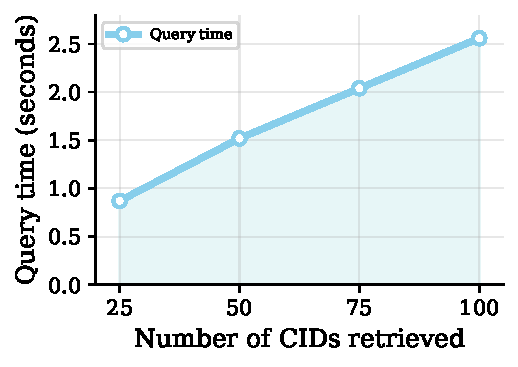
\includegraphics[width=\linewidth]{performance_evaluation_four_panels_c.pdf}
        \caption{Scalability vs CIDs}
        \label{fig:fig4c}
    \end{subfigure}
    \hfill
    % Subfigure (d)
    \begin{subfigure}[b]{0.24\linewidth}
        \centering
        
\includegraphics[width=\linewidth]{performance_evaluation_four_panels_d.pdf}
        \caption{Network Distribution}
        \label{fig:fig4d}
    \end{subfigure}
    
    \caption{Query efficiency of \ours under varying configurations. (a) Query latency with index remains nearly constant across database sizes. (b) without index, latency increases linearly. (c) Query time scales linearly with the number of matched partitions (CIDs). (d) Network distribution analysis shows latency increases with remote data retrieval, especially over WAN.}
    \label{fig:combined_evaluation}
\end{figure*}

% Now you can reference individual subfigures like this:
% As shown in \Cref{fig:fig4a}, indexing significantly reduces latency. 
% \Cref{fig:fig4b} shows the performance degradation without indexing.
% The scalability analysis in \Cref{fig:fig4c} demonstrates linear growth.
% Network effects are analyzed in \Cref{fig:fig4d}.
